\chapter{State of art}
In this chapter is presented the current implementation to support edge and fog computing paradigms within the energy production and monitoring network, based on the Smart Grid model (translating hardware components into an IT network) and the use of the Kubernetes platform. The limitations that the implementation studied in this thesis aims to eliminate will also be highlighted.

\section{Smart Grid components}
Currently, the Smart Grid model of the energy monitoring network consists of the Area Control Center, which is the central hub for control and decision-making mechanisms, and the production and distribution stations, which are divided into primary and secondary. 

To manage the network, three main applications are used: Phasor Measurement Units (PMU) for measurements, Phasor Data Concentrator (PDC) from the openPDC project for aggregating data from various PMUs, and Grid State Estimation (GSE) for monitoring the network based on the data provided by the previous applications. 

A graphical example of the Smart Grid model is shown in the Figure~\ref{fig:art-state}.
\begin{figure}[ht]\centering
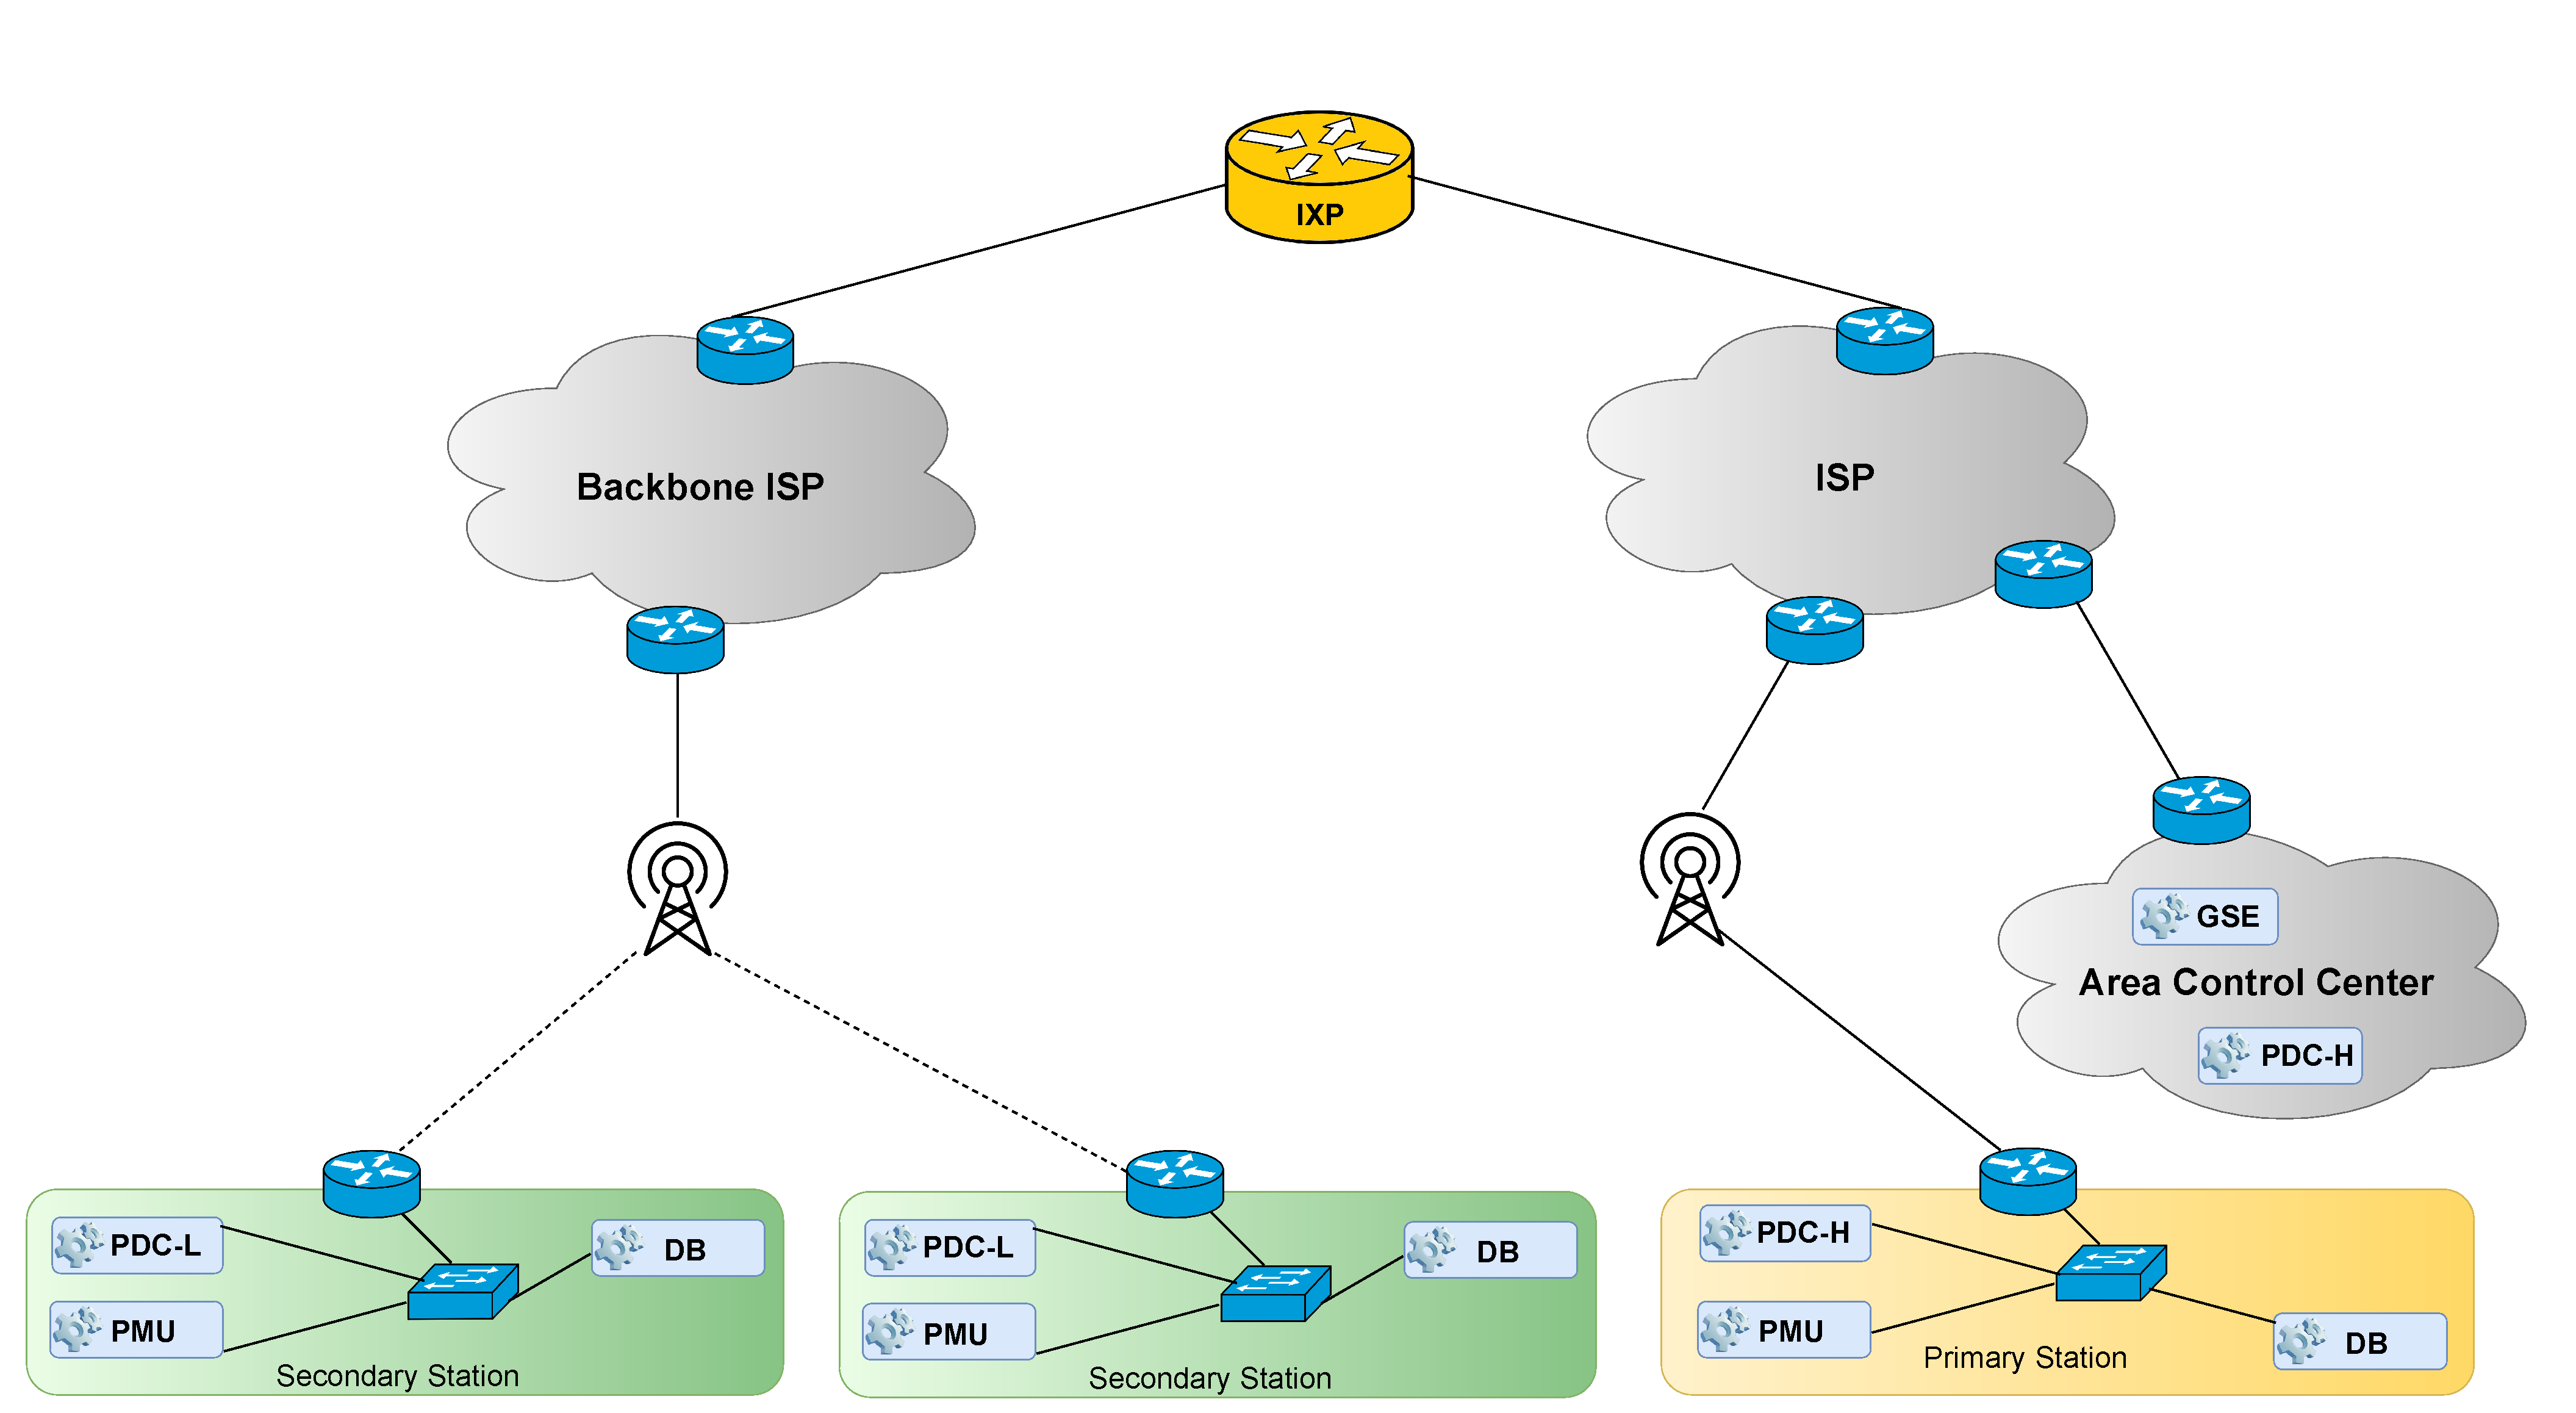
\includegraphics[scale=0.17]{Pictures/state-of-art}
\caption{Smart Grid abstract informatic model}\label{fig:art-state}
\end{figure}

\subsection{Area Control Center}
A computing node within the context of the Smart Grid that serves as an Operational Distribution Center, housing the control and management logic for the entire network.

This node is primarily responsible for overseeing the high-level PDC, where data streams from other high-level PDCs situated at primary stations are aggregated. Additionally, it manages the GSE application, which utilizes data from the aforementioned PDC to control the network.

\subsection{Station}
In the context of the Smart Grid, it is a computing node that represents an energy production or distribution station.

Primary stations typically utilize a high-level PDC to aggregate data streams from their subnet of secondary stations. Additionally, they may manage a certain number of PMUs (Phasor Measurement Units).

Secondary stations primarily handle PMUs or aggregate data streams generated by them through low-level PDCs.

\subsection{Phasor Measurement Units}
PMUs provide measurements of fundamental electrical quantities, such as voltage and current, in the form of phasors, including information on the amplitude and phase of the measured quantities. 

These measurements, synchronized via GPS and sampled at a frequency of 50 samples per second, enable precise monitoring of rapid changes in the electrical system caused by the dynamism of distributed energy resources.

PMUs offer a detailed perspective of system dynamics, overcoming the limitations of more traditional Remote Terminal Units (RTUs), which have an update period of several seconds and are not synchronized. The use of PMUs is expected to enhance the observability and reliability of the distribution system.

\subsection{Phasor Data Concentrator}
A phasor data concentrator (PDC) is designed to receive streaming synchrophasor data from phasor measurement units (PMUs) installed on power transmission lines and align these data using GPS timestamps (i.e., it "concentrates" the data based on time). 

The output of a PDC is a time-synchronized data set that is forwarded to one or more software applications.

openPDC is a flexible platform for high-speed time-series data processing, both in real-time and historically. It does not have significant computational power requirements, so it can be installed anywhere within the synchrophasor infrastructure, including on fanless computers located in substations.

\subsection{Grid State Estimation}
State estimation is a technique that allows for the reconstruction of network states, such as nodal voltages, based on available measurements and the electrical network model. Unlike traditional meters, PMU measurements, which include the phase relative to an absolute reference, simplify the state estimation problem by making it a linear system and significantly reducing the computational load. 

The objectives of state estimation include the recognition and reduction of measurement errors, the identification of topology errors, the estimation of unmeasured network quantities, and the determination of network parameters through redundant measurements.

\section{Multi-master station architecture}
Recent research has progressed towards managing individual locations such as stations within the Smart Grid using a multi-master architecture \cite{a2-1}\cite{a2-2}. This approach leverages enhanced resilience, allowing the system to withstand the failure of a master node. However, it comes with the trade-off of requiring additional resources for replicated control-plane components.

Within the cluster, application configurations (such as those for a PDC if the cluster represents a station) are stored in a high-availability distributed database system. This setup facilitates rapid and automatic redeployment to another node within the cluster in case of a failure, without needing to reconfigure the application parameters.

Consequently, the clusters support autonomous local recovery from both application and node failures.

Each cluster serves as a point of edge (for managing secondary stations) or fog (for managing primary stations) computing within the Smart Grid, depending on its location. However, the overall control architecture is manually established between each pair of clusters, each of which operates as a fully independent entity.

This manual establishment of control logic between clusters exhibits limited resilience due to potential errors in configuration and vulnerability in handling failures, while also presenting challenges in scalability.

\section{Actual limitations}
While this approach of a multi-cluster kubernetes is effective for managing a single station, it proves suboptimal when applied to an entire electrical control system.

This is due to both the complexity involved in managing a large number of nodes (with stations alone numbering in the tens of thousands, whereas Kubernetes officially supports up to 5000 nodes \cite{a3-1}) and the fundamental inability to function in isolation. 

Consider the possible failures that can occur within the architecture, as shown in Figure~\ref{fig:a-failures}. Despite there being no unrecoverable failures, since it functions as a single large Kubernetes cluster where deployments are not concentrated in one location and therefore continue to operate, any part that becomes disconnected from the network will no longer be controllable. 

This is because the master nodes on the isolated network loses the necessary consensus to initiate new workloads (new pods to manage the isolated entities) and can only partially manage existing workloads (because it can't reschedule workloads if it fails).

\begin{figure}[ht]\centering
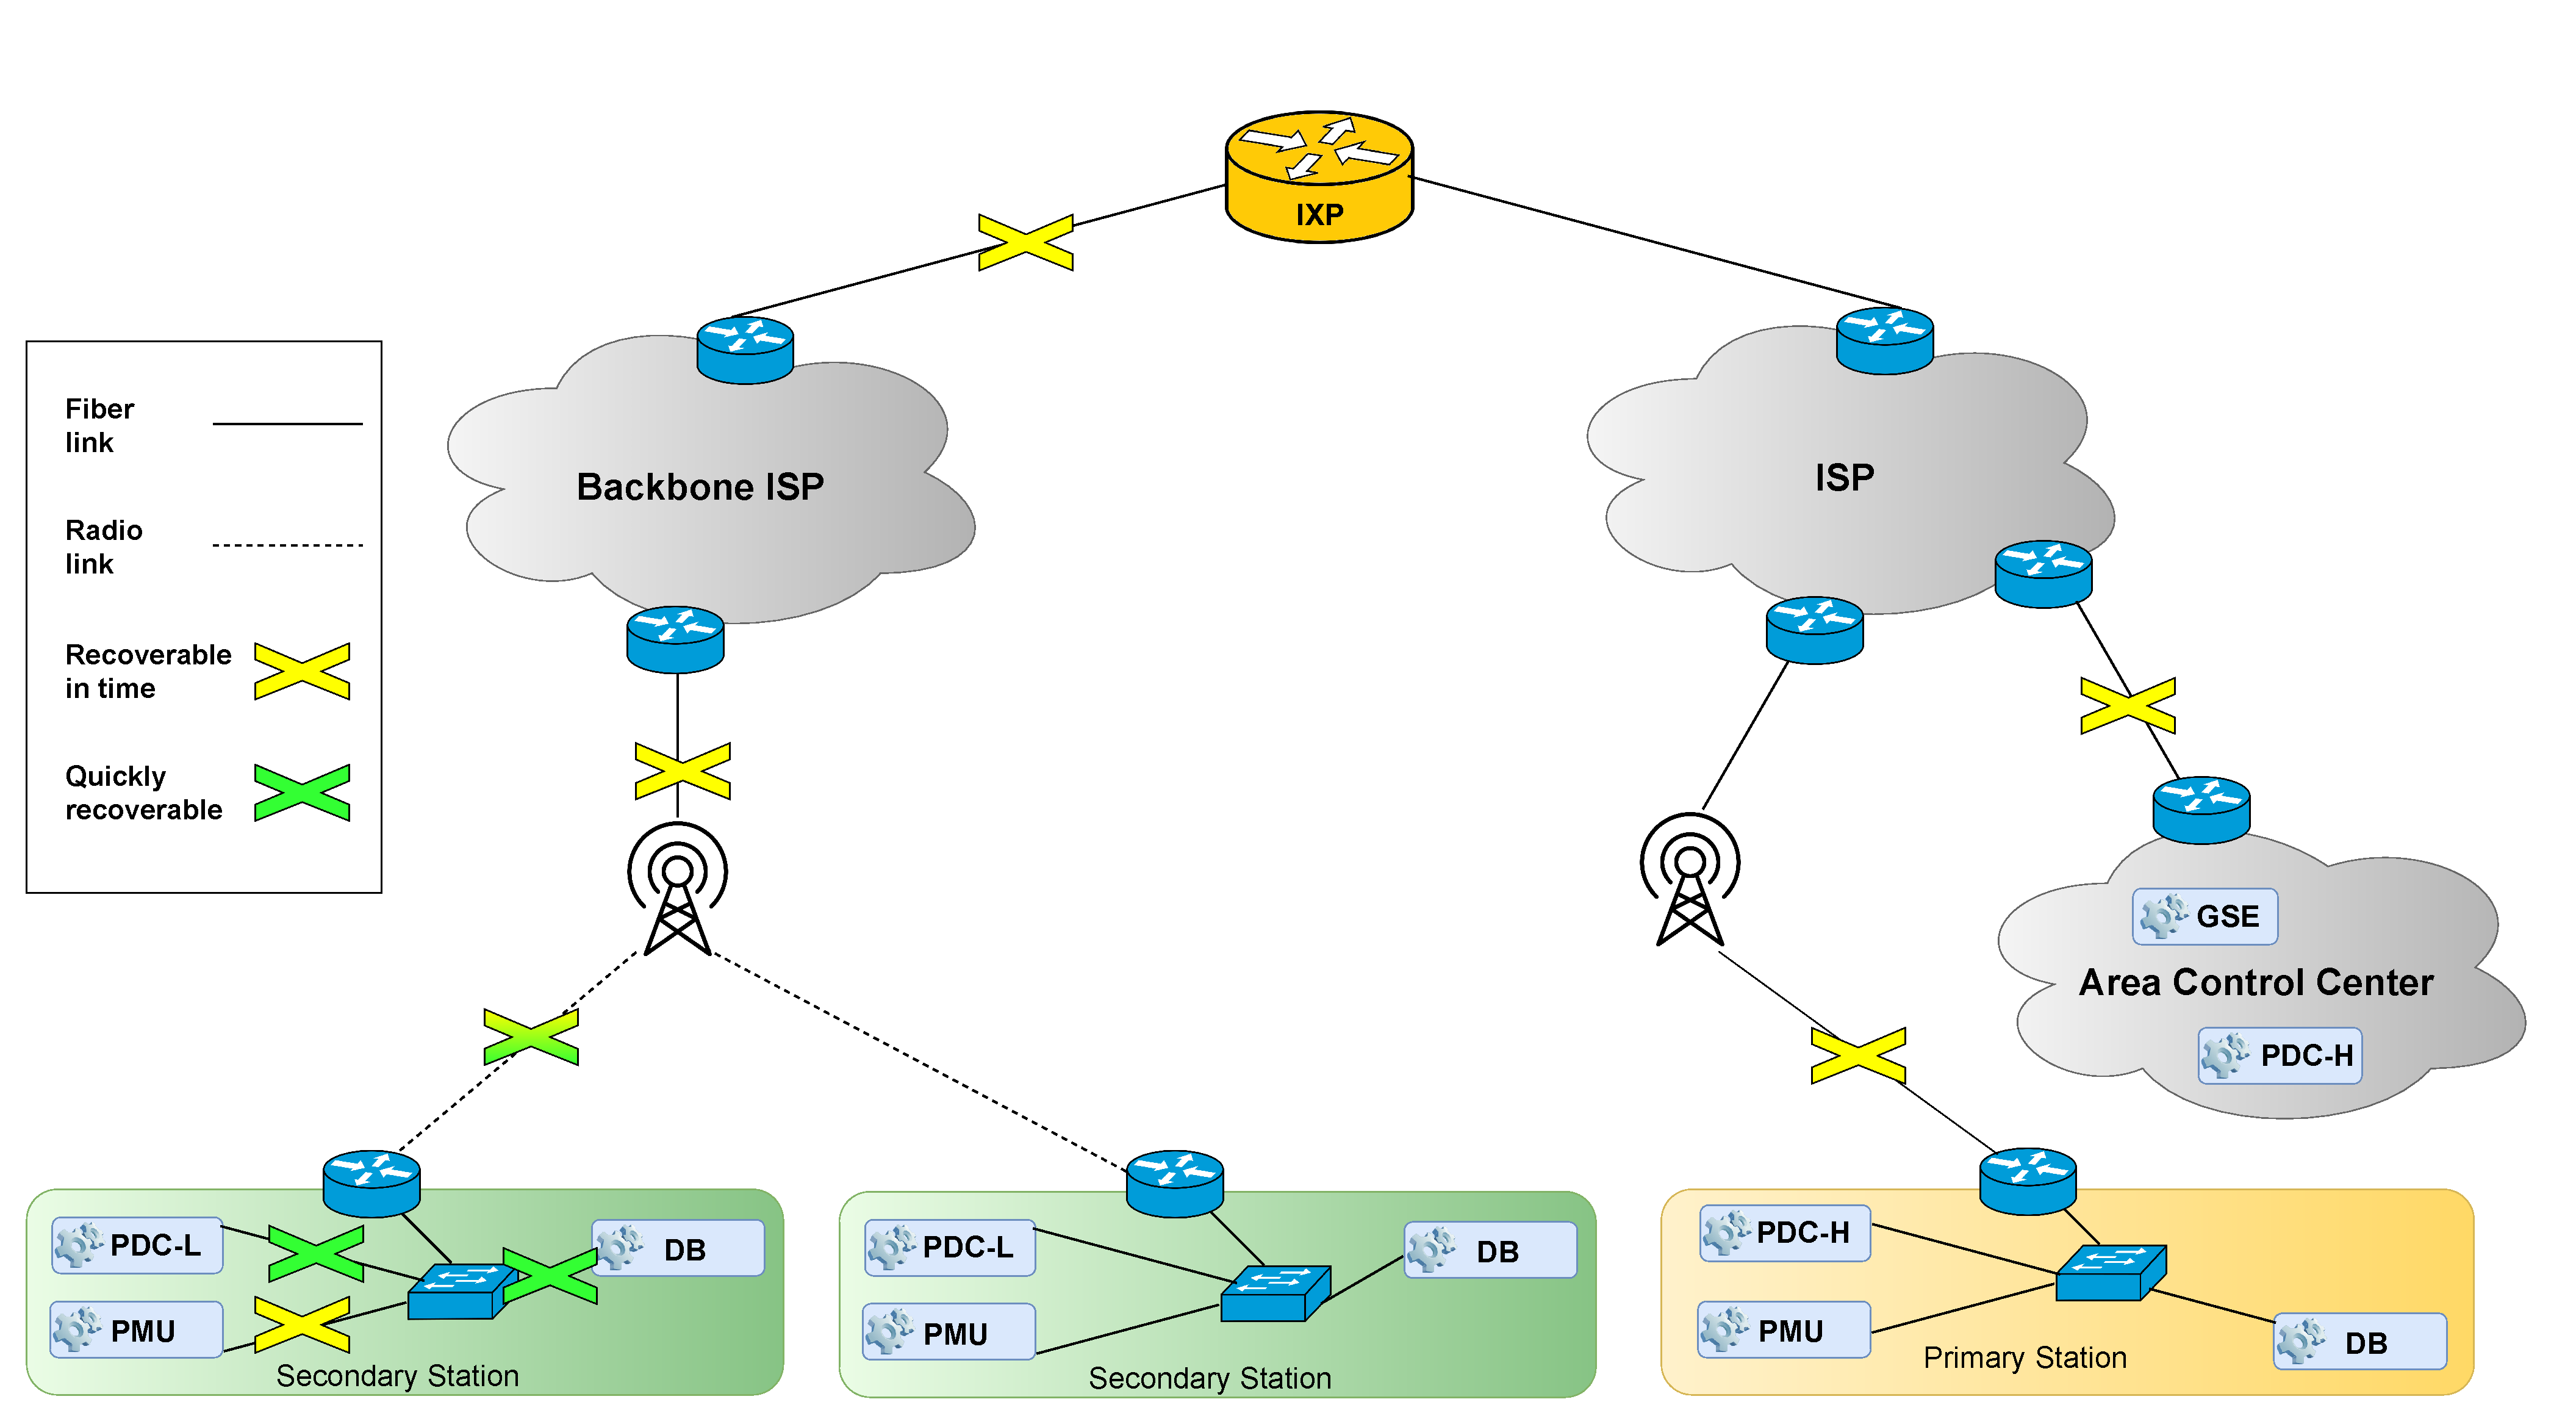
\includegraphics[scale=0.20]{Pictures/actual-failures}
\caption{Possible failures in multi-level logical domains implementation}\label{fig:a-failures}
\end{figure}

The only additional failure scenario that the translated architecture (from local environment to the entire network) can address without losing the ability to control is when an entire secondary station without source data but with the aggregator applicative becomes isolated from the network, because it simply transfer the PDC to another healty node.

However, this advantage does not outweigh the drawbacks in terms of complexity,lack of scalability, and resource demands inherent in the overall architecture. 

An additional limitation concerns the number of master nodes that must necessarily remain healthy. Considering a cluster at its maximum size (which has already been shown to be insufficient to cover an entire network), the highest resilience is achieved with 7 master nodes. In this case, the architecture continues to function as long as 4 out of the 7 master nodes remain active.

These limitations can be effectively addressed by adopting Liqo technology. For instance, instead of needing 4 nodes to remain active, only one node, the one representing the Area Control Center, needs to stay operational.